\DeclareOldFontCommand{\bf}{\normalfont\bfseries}{\mathbf}
\documentclass[
	fontsize=12pt,
	paper=a4,
	bibliography=totoc,
	index=totoc,
	listof=totoc,
	footinclude=false,
	BCOR16mm,
	DIV=10
	]{scrbook}


%%%%% include settings
% Included by MAIN.TEX
% Defines the settings for the CAMP report document

% use german characters as well
\usepackage[utf8]{inputenc}       % allow UTF-8 characters
%\usepackage[ansinew]{inputenc}       % allow ANSII-new characters

\renewcommand{\sectfont}{\normalfont \bfseries}        % Schriftart der Kopfzeile

% manipulate footer
\usepackage{scrpage2}
\pagestyle{scrheadings}
\ifoot[\footertext]{\footertext} % \footertext set in INFO.TEX
%\setkomafont{pagehead}{\normalfont\rmfamily}
\setkomafont{pagenumber}{\normalfont\rmfamily}


%\usepackage{algorithm}
%\usepackage{algpseudocode}
%\floatname{algorithm}{Algorithmus}
%\usepackage{framed}
%\usepackage{multicol}

%% allow sophisticated control structures
\usepackage{ifthen}

% use Palatino as default font
\usepackage{palatino}

% enable special PostScript fonts
\usepackage{pifont}

%to use the subfigures
\usepackage{subfigure}

%\usepackage{wrapfig}
\usepackage{listings}
\usepackage{color}
\usepackage[svgnames]{xcolor}
\usepackage{colortbl}

% for js listings
\usepackage{caption}
\usepackage{jslistings}

\usepackage{url}
\usepackage{stackengine}

%\makeatletter 
%\g@addto@macro\UrlBreaks{ 
%  \do\a\do\b\do\c\do\d\do\e\do\f\do\g\do\h\do\i\do\j 
%  \do\k\do\l\do\m\do\n\do\o\do\p\do\q\do\r\do\s\do\t 
%  \do\u\do\v\do\w\do\x\do\y\do\z\do\&\do\1\do\2\do\3 
%  \do\4\do\5\do\6\do\7\do\8\do\9\do\0} 
%% \def\do@url@hyp{\do\-} 
%\makeatother 

\usepackage{url}
\urlstyle{same}

%% show program code\ldots
%\usepackage{verbatim}
%\usepackage{program}

%% enable TUM symbols on title page
\usepackage{styles/tumlogo}


\usepackage{multirow}

%% use colors
\usepackage{color}

%% make fancy math
\usepackage{amsmath}
\usepackage{amsfonts}
\usepackage{amssymb}
\usepackage{textcomp}
\usepackage{yhmath} % f�r die adots 
%% mark text as preliminary
%\usepackage[draft,german,scrtime]{prelim2e}

%% create an index
\usepackage{makeidx}

% for the program environment
%\usepackage{float}
\usepackage{tocbasic}

%% load german babel package for german abstract
%\usepackage[german,american]{babel}
\usepackage[ngerman]{babel}
%\selectlanguage{german}

% use initals dropped caps - doesn't work with PDF
%\usepackage{dropping}


\usepackage{styles/shortoverview}
%----------------------------------------------------
%      Graphics and Hyperlinks
%----------------------------------------------------


%% check for pdfTeX
\ifx\pdftexversion\undefined
 %% use PostScript graphics
 \usepackage[dvips]{graphicx}
 \DeclareGraphicsExtensions{.eps,.epsi}
 \graphicspath{{figures/}{figures/review}} 
 %% allow rotations
 \usepackage{rotating}
 %% mark pages as draft copies
 %\usepackage[english,all,light]{draftcopy}
 %% use hypertex version of hyperref
 \usepackage[hypertex,hyperindex=false,colorlinks=false,breaklinks]{hyperref} 
 %% breaks urls if they are too long
 \usepackage{breakurl}
\else %% reduce output size \pdfcompresslevel=9
 %% declare pdfinfo
 %\pdfinfo { 
 %  /Title (my title) 
 %  /Creator (pdfLaTeX) 
 %  /\dfrac{Author}{den} (my name) 
 %  /Subject (my subject	) 
 %  /Keywords (my keywords)
 %}
 %% use pdf or jpg graphics
 \usepackage[pdftex]{graphicx}
 \DeclareGraphicsExtensions{.jpg,.JPG,.png,.pdf,.eps}
 \graphicspath{{figures/}} 
 
 %% allow rotations
 \usepackage{rotating}
 %% use pdftex version of hyperref
 \usepackage[pdftex,colorlinks=true,linkcolor=black,citecolor=black,%
 anchorcolor=black,urlcolor=black,bookmarks=true,%
 bookmarksopen=true,bookmarksopenlevel=0,plainpages=false,%
 bookmarksnumbered=true,hyperindex=false,pdfstartview=%
 ]{hyperref}
%
%\usepackage[pdftex,colorlinks=false,linkcolor=red,citecolor=red,%
% anchorcolor=red,urlcolor=red,bookmarks=true,%
% bookmarksopen=true,bookmarksopenlevel=0,plainpages=false%
% bookmarksnumbered=true,hyperindex=false,pdfstartview=%
% ]{hyperref}




%% Fancy chapters
%\usepackage[Lenny]{fncychap}
%\usepackage[Glenn]{fncychap}
%\usepackage[Bjarne]{fncychap}

%\usepackage[avantgarde]{quotchap}

% set the bibliography style
\bibliographystyle{unsrtnat}

\usepackage{textcomp}
%\definecolor{listinggray}{gray}{0.9}
%\definecolor{lbcolor}{rgb}{0.9,0.9,0.9}
%\lstset{language=XML}

\usepackage[all]{hypcap}
\pdfminorversion=6

\usepackage[T1]{fontenc}
\usepackage{epsfig}
\usepackage[numbers,sort&compress]{natbib}
\usepackage{bm}
\usepackage[normalem]{ulem}

%% Do tabs
\usepackage{tabto}

\addtokomafont{captionlabel}{\bfseries}

%% Use enumeration of subsubsections
\setcounter{secnumdepth}{3}

%% Use footnote numbering for whole document
\usepackage{chngcntr} 
\counterwithout{footnote}{chapter}

\DeclareNewTOC[
    counterwithin=chapter,
    float, type=codelisting, types=codelistings,
    name={Listing}, listname={List of Code}
]{loc}
\setuptoc{loc}{chapteratlist}

%% \DeclareNewTOC[%
%	counterwithin=chapter,%
%	hang=2em,%
%	type=example,%
%	types=examples,%
%	nonfloat,%
%	name=Beispiel,%
%	listname={Beispielverzeichnis}%
%]{loex}
%\setuptoc{loex}{chapteratlist}

%\DeclareNewTOC[%
%	counterwithin=chapter,%
%	hang=2em,%
%	type=definition,%
%	types=definitions,%
%	nonfloat,%
%	name=Begriff,%
%	listname={Begriffsverzeichnis}%
%]{lode}
%\setuptoc{lode}{chapteratlist}

%\setlength{\textfloatsep}{-20pt}
%\setlength{\belowcaptionskip}{10pt plus 0pt minus 0pt}

%%%%% include command
% Commands to be used within the TUM report document
% Included by MAIN.TEX
% Please include your own cool commands here. 
% Be only sure to comment it sufficiently so others can use it.

%-------------------------------------------------------------
%                      Own Commands
%-------------------------------------------------------------


%-------------------------------------------------------------
% math stuff -------------------------------------------------

% nice R, N, C
\newcommand{\nat}{\mathbb{N}}
\newcommand{\real}{\mathbb{R}}
\newcommand{\compl}{\mathbb{C}}



% norm
\newcommand{\norm}[1]{\left\| #1 \right\|}

% un demi
\newcommand{\half}{\frac{1}{2}}

% parantheses
\newcommand{\parenth}[1]{ \left( #1 \right) }
\newcommand{\bracket}[1]{ \left[ #1 \right] }
\newcommand{\accolade}[1]{ \left\{ #1 \right\} }
%\newcommand{\angle}[1]{ \left\langle  #1 \right\rangle }

% partial derivative: %#1 function, #2 which variable
% simple / single line version
\newcommand{\pardevS}[2]{ \delta_{#1} f(#2) }
% fraction version
\newcommand{\pardevF}[2]{ \frac{\partial #1}{\partial #2} }

% render vectors: 3 and 4 dimensional
\newcommand{\veciii}[3]{\left[ \begin{array}[h]{c} #1 \\ #2 \\ #3	\end{array} \right]}
\newcommand{\veciv}[4]{\left[ \begin{array}[h]{c} #1 \\ #2 \\ #3 \\ #4	\end{array} \right]}

% render matrices: 3  dimensional (arguments in row first order)
\newcommand{\matiii}[9]{\left[ \begin{array}[h]{ccc} #1 & #2 & #3 \\ #4 & #5 & #6 \\ #7 & #8 & #9	\end{array} \right]}
%DOESN'T WORK,DON'T KNOW WHY \newcommand{\mativ}[16]{\left[ \begin{array}[h]{cccc} #1 & #2 & #3 & #4 \\ #5 & #6 & #7 & #8 \\ #9 & #10 & #11 & #12 \\ #13 & #14 & #15 & #16 \end{array} \right]}


%-------------------------------------------------------------
%-------------------------------------------------------------


%-------------------------------------------------------------
% some abreviations ------------------------------------------
\newcommand{\Reg}{$^{\textregistered}$}
\newcommand{\reg}{$^{\textregistered}$ }
\newcommand{\Tm}{\texttrademark}
\newcommand{\tm}{\texttrademark~}
\newcommand {\bsl} {$\backslash$}

%-------------------------------------------------------------
%-------------------------------------------------------------



%-------------------------------------------------------------
% formating --------------------------------------------------

% Theorem & Co environments and counters
%\newtheorem{theorem}{Theorem}
%\newtheorem{lemma}[theorem]{Lemma}
%\newtheorem{corollary}[theorem]{Corollary}
%\newtheorem{remark}[theorem]{Remark}
%\newtheorem{definition}[theorem]{Definition}
%\newtheorem{equat}[theorem]{Equation}
%\newtheorem{example}[theorem]{Example}
% \newtheorem{algorithm}[theorem]{Algorithm}

% inserting figures
%\newcommand{\insertfigure}[4]{ % Filename, Caption, Label, Width percent of textwidth
%	\begin{figure}[htbp]
%		\begin{center}
%			\includegraphics[width=#4\textwidth]{#1}
%		\end{center}
%		\vspace{-0.4cm}
%		\caption{#2}
%		\label{#3}
%	\end{figure}
%}

%-------------------------------------------------------------
%-------------------------------------------------------------


% new stuff (Michael)

%-------------------------------------------------------------
%-------------------------------------------------------------

\newcommand{\insertfigure}[3]{ %filename and label, width, caption
	\begin{figure}
		\center
		\includegraphics[width=#2\columnwidth]{images/#1}
		\vspace{-0.2cm}
		\caption{#3}
		\label{fig:#1}
	\end{figure}
}

\newcommand{\insertdefinition}[3] { %label, caption, text
%	\begin{definition-}
		\KOMAoptions{captions=nooneline}
		\captionof{definition}[#2]{\textbf{#2}: #3}
		\label{def:#1}
		\vspace{0.2cm}
		\KOMAoptions{captions=oneline}
%	\end{definition-}
}

\newcommand{\insertexample}[3] { %label, caption, text
	\begin{example-}
		\KOMAoptions{captions=nooneline}
		\captionof{example}[#2]{\textbf{#2}:}
		\label{ex:#1}
		\KOMAoptions{captions=oneline}
		\setlength\parindent{1em}
		#3
	\end{example-}
}

\newcommand{\insertlst}{
	\lstset{
		basicstyle=\small,
		keywordstyle=\bfseries,
		commentstyle=\color{green!50!black!100}, 
		stringstyle=\ttfamily, 
		language=Java,                % choose the language of the code
		frame=single,	                % adds a frame around the code
		aboveskip=11pt,
		belowskip=11pt,
		breaklines=true,                % sets automatic line breaking
		breakatwhitespace=false,  % sets if automatic breaks should only happen at
		showspaces=false,
		showstringspaces=false
	}
}



% Set here the title, authors and other stuff to be used for the cover
% This file is used by MAIN.TEX



% set title, authors and stuff for the cover
\def\doctype{Master Thesis}
\def\title{Offline caching in web applications for AntidoteDB} 
\def\author{Server Khalilov}
\def\date{15. December 2018}

% text to appear in the footer
\def\footertext{}


%%%%% global hyphenation
\hyphenation{
}

\sloppy

\makeglossary

\begin{document}
\renewcommand{\chaptername}{Chapter}
\renewcommand\contentsname{Contents}
\renewcommand{\tablename}{Table}
\renewcommand{\listtablename}{List of Tables}
\renewcommand{\figurename}{Figure}
\renewcommand{\listfigurename}{List of Figures}
\renewcommand{\bibname}{Bibliography}
\renewcommand{\appendixname}{Appendix}

	%%%%% Deckblatt
	\frontmatter	
	% The front cover for the TUM report document.
% Included by MAIN.TEX


%--------------------------------------------------
% The Front Cover
%--------------------------------------------------

% The front cover for the TUM document.
% Included by MAIN.TEX


%--------------------------------------------------
% The Front Cover
%--------------------------------------------------

% correct BCOR - undo at the end !!!
\def\bcorcor{0.15cm}
\addtolength{\hoffset}{\bcorcor}

\thispagestyle{empty}

 \vspace{4cm}
\begin{center}
	     %  \oTUM{4cm}
	   
	   \vspace{5mm}     
	   \large Department of Computer Science\\ 
	   \vspace{0.5cm}
	 \large University of Kaiserslautern\\
    \vspace{1mm}
        
	\end{center}
		

\vspace{20mm}
\begin{center}

   {\LARGE \doctype}

  \vspace{15mm}  
  {\huge\textbf \title\par}%[3ex]
  
  
  \vspace{20mm}
   
  {\LARGE  \author}
  
  \vspace{10mm}
	
%	xxx@cs.uni-kl.de\\
	University of Kaiserslautern\\
	Department of Computer Science\\
	Software Engineering\\
	\ \\
	Leader:\\
	Prof. Dr. Arnd Poetzsch-Heffter\\
	\ \\
	Supervisor:\\
	Dr. rer. nat. Annette Bieniusa\\
  
%  \includegraphics[width=8cm]{images/Marimba}
  
  \vspace{10mm}
  
  
\includegraphics[width=4cm]{styles/tulogo}
  
  \end{center}
	
	%%%%% Abstract und Disclaimer
	\cleardoubleoddemptypage
	\thispagestyle{plain}
	% German abstract for the CAMP report document
% Included by MAIN.TEX

\begin{center}
{\Large \textbf Zusammenfassung}
\end{center}
\vspace{1cm}

Zusammenfassung auf deutsch
	\cleardoubleoddplainpage
	% Abstract for the TUM report document
% Included by MAIN.TEX

\begin{center}
{\Large \textbf Abstract}
\end{center}
\vspace{1cm}


The goal of this thesis is to design a web-client for Antidote-DB with a support of caching with a further implementation. In order to achieve this goal, the understanding of how CRDT works needs to be reached. The paper could be logically divided into two parts: firstly, the problem of designing mentioned solution is going to be discussed. Secondly, there is an implementation part and description how specific problems were tackled.
	
	\cleardoubleevenplainpage
	% Abstract for the TUM report document
% Included by MAIN.TEX

\begin{center}
{\Large \textbf Acknowledgement}
\end{center}
\vspace{1cm}

I would like to take this opportunity and express my biggest gratitude to everyone, who supported me through all the ups and downs I had during my time at the Univesity of Kaiserslautern. 

Firstly, I am very grateful to \textbf{Prof. Dr. Arnd Poetzsch-Heffter} and my thesis supervisor \textbf{Dr. rer. nat. Annette Bieniusa} for making it possible for me to work on the topic that suits my area of interest. Moreover, I want to thank Annette for having the door to her office always open for a discussion, whenever I needed it. I am happy I had a chance to work with her on multiple occasions: firstly, during the time of the lecture on Compiler and Language-Processing Tools; then, while being a research assistant in EU Project "Lightkone"; and, finally, by writing a Master's thesis under her guidance. She was always patient and continuously motivated me to strive for better results. I could not ask for more.

Next, I would like to thank the stuff at Software Technology Group, who made me feel very welcome and patiently answered any questions I had. Especially, \textbf{Mathias Weber}, \textbf{Peter Zeller}, and \textbf{Deepthi Akkoorath}.

Finally, I want to mention my friends, family and, particularly, \textbf{my parents} and \textbf{sister}. They did their very best to encourage and motivate me throughout the whole period of my study in Germany. Nothing of it would ever be possible without them. Thank you.

	\cleardoubleevenplainpage
	%\selectlanguage{german}
	\vspace*{0.72\textheight}
	\noindent
Ich versichere hiermit, dass ich die vorliegende Masterarbeit mit dem Thema
"`\title"' selbstständig verfasst und keine anderen als die angegebenen Hilfsmittel benutzt habe. \\
Die Stellen, die anderen Werken dem Wortlaut oder dem Sinn nach entnommen wurden, habe ich durch die Angabe der Quelle kenntlich gemacht.
	
	\vspace{8mm}
	\noindent
	Kaiserslautern, den \date \hspace{3,5cm} \author
%\selectlanguage{english}
\newpage
	
	%%%%% Inhaltsverzeichnis
	\cleardoubleoddplainpage
	\pdfbookmark[1]{Contents}{toc}
	{\hypersetup{linkcolor=black}
	\tableofcontents
	}
	
	%%%%% Alle anderen Kapitel, Anhang und Verzeichnisse
	\mainmatter

		\cleardoubleoddplainpage
		\label{part:Introduction}
		\chapter{Introduction}
\label{Introduction}

In this chapter we are going to discuss the motivation, research questions and the scope of this thesis.

o Problem context (What is the broader context of this work?) 
o Problem description (What is the specific problem or challenge addressed by this work?) 
o Research question(s) (What are the actual questions that should be answered by this research? Why are they interesting? To whom? Why is there no obvious answer? If this is getting too much, then details of discussion can be deferred until later, e.g., to the methodology section.) 
o Summary of results and contributions (What is the outcome of this work in simple terms?) 
o Structure of the thesis (Introduce briefly the remaining chapters.)

\section{Motivation}

The motivation of this thesis is to explore the possibilities of implementing a web-client with a cache on a client-side. 

\section{Research questions}

The following research questions are going to be addressed in this thesis:
\\\\
\textbf{RQ1.} How efficient is it to use a web-client with cache rather than without it?
\\\\
\textbf{RQ2.} What are the methods available to implement web-applications that would be able to work off-line and in the conditions of poor network connections?
\\\\
\textbf{RQ3.} What could be a scalable solution for transmitting CRDT data between a server and clients?

		\cleardoubleoddplainpage
		\label{part:Background}
		\chapter{Theoretical background}
\label{Background}

In this chapter, we are going to introduce the reader to the theoretical concepts, which represent a prerequisite to have an understanding of this thesis.

\section{Main concepts}
\label{Background-Main}

\textit{Distributed database} is ``a collection of multiple, logically interrelated databases distributed over a computer network''\cite{11}. A \textit{geo-distributed database}, in its turn, is a database, which is spread across two or more geographically distinct locations and runs without experiencing performance delays. The maintaining of such databases brings its challenges. As the database is spread across several locations, there should be a replication process in order to ensure that replicas of that database synchronise and have the latest state of the data. This replication process should be fast, because if there are two replicas of the database, then whenever there is some information written to the first replica, it should be accessible to users, who use the second one. That is the problem of the availability, but before the information at replicas becomes available, it first should be checked over the consistency, as the states of the replicas should be equal. That is a complex task to solve. 

Working with such a distributed database, whenever the data is needed to be read or changed in any way, a transaction should be started, executed and closed. A \textit{transaction} is a basic unit of computing, which consists of a sequence of operations that are applied atomically on a database. Transactions transform a consistent database state to another consistent database state. A transaction is considered to be \textit{correct} if it obeys the rules, specified on the database. As long as each transaction is correct, a database guarantees that concurrent execution of user transactions will not violate database consistency \cite{11}. \textit{Consistency} requires transactions to change the data only according to the specified rules. An example of consistency rule can be the following: let us say that in a bank database the bank account number should only consist of integer numbers. If an employee tries to create an account that contains something other than integer numbers in it, then the database consistency rule will disallow it. Consistency rules are important as they control the incoming data and reject the information, which does not fit.

\textit{Sequential consistency} and \textit{linearizability} are two consistency conditions that are well-known. Sequential consistency requires that all of the data operations appear to have executed atomically (i.e. independently), in some sequential order. When this order must also preserve the global ordering of non-overlapping operations, this consistency is called linearizability\cite{27}. Linearizability guarantees that the same operations are applied in the same order to every replica of the data item\cite{12}. Serializability is a guarantee about transactions, that they are executed serially (i.e. without overlapping in time) on every set of the data items\cite{12}. Serializability is more strict than sequential consistency, as the granularity of sequential consistency is a single operation, while for serializability it is a transaction. As a result, when serializability is satisfied, the sequential consistency is also satisfied, but not vice versa.

Now, let us introduce different consistency models and the one we will follow in the designing part of WebCure. 

As stated by \citet{10}, ``\textit{strong consistency} model could be described in the following way: whenever the update is performed, everyone knows about it''. It means that there is a total order of updates, and reads are guaranteed to return the latest data, regardless of which replica is the source of the response. The advantage of strong consistency is that the database is always in a consistent state and to disadvantages, we can add low latency, as there is a delay for making sure that all the replicas are in a consistent state before any other read / write requests could be processed. The latency point is a huge drawback for the performance, especially if a strong consistency model is considered to be used as a solution for the web, where users usually expect high responsiveness and availability. 

The main point of replicating data is to improve such aspects as reliability, availability, performance and latency. However, according to CAP Theorem\cite{29}, a distributed database can only have two of the three properties: consistency, availability and partition tolerance. This theorem is fundamental, as it makes people think towards the trade-off between those three properties for a specific use case. There are some weaker consistency models, where the results of requests can alter depending on the replica\cite{28}.  In this thesis, we will stick with partial \textit{causal consistency}. As it is stated in \citet{7}, causal consistency is ``the strongest available and convergent model''. They continue their statement saying that ``under causal consistency, every process observes a monotonically non-decreasing set of updates that includes its updates, in an order that respects the causality between operations''. As the causal ordering is respected, it makes it easier for programmers to reason, as it gives the guarantee that related events are visible in the order of occurrence, while the events, which have no relation to each other, can be in a different order in different replicas. Let us consider an example of an application for some of social networks. There, a reply to a wall post happens after the original post is published. Thus, users should not see the reply before the original post is observable. This type of guarantees is provided by causal consistency. Looking at \figref*{fig:theory3} we can see that on the left subfigure, the user can see the original wall post as well as the reply, while on the right subfigure, without causal consistency, the user sees only the reply, while the original wall post is missing. 

\begin{figure}%
    \centering
    \def\svgwidth{0.4\linewidth}
    \subfloat[]{{\input{images/causal/causal_true.pdf_tex}}}%
    \qquad
    \def\svgwidth{0.4\linewidth}
    \subfloat[]{{\input{images/causal/causal_false.pdf_tex}}}%
    \caption{An example of how a causally consistent behaviour (a) and the one that is not (b) could work in a social network.}%
    \label{fig:theory3}%
\end{figure}





\section{AntidoteDB}
\label{2-antidotedb}

For this thesis, one of the core parts of the architecture of WebCure belongs to the database called AntidoteDB\cite{4}. It helps programmers to write correct applications and has the same performance and horizontal scalability as AP / NoSQL\cite{14}, while it also:

\begin{itemize}
\item {is geo-distributed, which means that the datacenters of AntidoteDB could be spread across anywhere in the world;}
\item {groups operations into atomic transactions\cite{9, 15};}
\item {delivers updates in a causal order and merges concurrent operations.}
\end{itemize} 

Merging concurrent operations is possible because of CRDTs\cite{2}, which are used in AntidoteDB. It supports counters, sets, maps, multi-value registers and other types of data that are designed to work correctly in the presence of concurrent updates and failures. The usage of CRDTs allows the programmer to avoid problems that are common for other databases like NoSQL, which are fast and available, but hard to program against\cite{15}. We will cover the topic of CRDTs later in this chapter.

Apart from that, to replicate the data AntidoteDB implements the \textit{Cure}\cite{15} protocol. It is a highly scalable protocol, which provides causal consistency. 

To ensure the guarantees it offers, AntidoteDB uses timestamps, indicating the time after the transaction. Timestamps are considered to be unique, totally ordered, and consistent with causal order, which means that if \textit{operation 1} happened before \textit{operation 2}, then the timestamp related to the \textit{operation 2} is greater than the one related to the \textit{operation 1}\cite{2}.Whenever the update operation has to be applied, it is also possible to provide a minimum time from what that update should be performed. This information is useful when a client is working with a server, which is based on AntidoteDB. In such cases, when one data centre stops working, the client can reconnect to another one. As a client can remember the latest timestamp for the data it has worked on, the failover to another data centre is possible without any additional efforts, as the timestamp information will help the client to request only the data, which have timestamps greater than the one, which is already stored at the client.

\section{CRDTs}
\label{2-crdts}

As it is stated in the work of \citet{3}, a CRDT is an abstract datatype, which is designed for a possibility to be replicated at multiple processes and possesses the following properties:


    \begin{itemize}
        \item {The data at any replica can be modified independently of other replicas;}
        \item {Replicas deterministically converge to the same state when they received the same updates.}
    \end{itemize}

Replication is a fundamental concept of distributed systems, well studied by the distributed algorithms community\cite{2}. There are two models of replication that are considered: state-based and operation-based. We are going to introduce our reader to both of them below. 

\subsection*{Operation-based replication approach}

\begin{figure}[!htb]
    \begin{center}
    \def\svgwidth{\linewidth}
    \input{images/crdts-replication/op-based.pdf_tex}
    \caption {Operation-based approach\cite{2}. <<S>> stands for source replicas and <<D>> for downstream replicas. }
    \label{fig:theory1}
\end{center}
\end{figure}

In this thesis, we are going to use the operation-based replication approach, where replicas converge by propagating operations to every other replica\cite{3}. Once an operation is received in a replica, it is applied locally. Afterwards, all replicas would possess all of the updates. In \figref*{fig:theory1}, we can see that firstly operations \textit{f(x\textsubscript{i})}, \textit{g(x\textsubscript{i})} applied locally at source replicas \textit{x\textsubscript{i}}, and then the operations are conveyed to all the other replicas. The second part of this process is named \textit{downstream} execution.

This replication approach infers that replicas do not exchange full states with each other, which is a positive concerning efficiency. Not always, though, as it depends on the task. Sometimes, applying multiple operations at every replica could be costly, and this is where state-based replication approach is beneficial.

% TODO What are the requirements for the op-based CRDTs to work correctly?
% Give an example of an op-based CRDT specification? counter!!!

\subsection*{State-based replication approach}
\begin{figure}[!htb]
    \begin{center}
    \def\svgwidth{\linewidth}
    \input{images/crdts-replication/state-based.pdf_tex}
    \caption {State-based approach\cite{2}. <<S>> stands for source replicas and <<M>> for merging stages.}
    \label{fig:theory2}
\end{center}
\end{figure}

The idea of this approach is kind of opposite to the operation-based one. Here, every replica, when it receives an update, first applies it locally. Afterwards, it sends its updated state to other replicas. Following this way, every replica sends its current full state to other replicas. Afterwards, the merge function is applied between a local state and a received state, and every update eventually is going to appear at every other replica in the system. We can see this it in the \figref*{fig:theory2}, where \textit{x\textsubscript{i}} stands for replicas, \textit{f(x\textsubscript{i})}, \textit{g(x\textsubscript{i})} stands for the functions that apply updates locally at source replicas before sending a new full state for a follow-up merges to other replicas in the system.

%What are the requirements for the state-based CRDTs to work correctly?

There are different types of CRDTs, yet, we will consider three of them: counters, sets and multi-value registers. We will give a brief description to each of the mentioned datatypes below.

\subsection*{Counter}

Counter is a datatype, which keeps track on its state, which is an integer number. The value of the Counter could be modified by the operations \textit{inc} and \textit{dec} that increases or decreases the state by one unit, accordingly\cite{3}. The concurrency semantics for this datatype is that a final state of the object reflects all the performed operations on it. In other words, to calculate the state of the Counter, it is needed to count the number of increments and subtract the number of decrements. 

\subsection*{Add-wins Set}

Add-wins Set\footnote{For the simplicity of reading, later it goes as Set.} datatype represents a collection of objects with a specific handling of concurrent updates performed over them. In case of concurrent updates on the same object, \textit{add} operations in Set win against \textit{remove} operations. If, for example, there is an empty set \textit{} and two concurrent operations applied to it -- \textit{add a} and \textit{remove a}, then the result is going to be \textit{\{a\}}, as \textit{add} operation wins. A \textit{remove} operation will ``overwrite'' an \textit{add} operation only when it happens after it\cite{3}. 

\subsection*{Multi-value Register}

This datatype maintains a value and provides a \textit{write} operation of updating that value. The exciting part about multi-value Registers is their concurrency semantics. In the case of two or more updates happening at the same time, all values are kept. Thus, the state of the register will consist of all the concurrently written updates for further processing. However, any additional single \textit{write} operation will overwrite the previous state of the register, even if it consisted of multiple values\cite{39}.
		
		\cleardoubleoddplainpage
		\label{part:Requirements}
		\chapter{Requirements}
\label{Requirements}

In this chapter, we will describe the requirements for the desired web-application. 

\section{Problem Description}

The application should showcase the functionality of communicating with an AntidoteDB database while online. As well as that, it should be reliable, which means it should load instantly and work even in uncertain network conditions. The application should be able to respond quickly to user interactions, be highly available (possible to work with it even when there is no internet at all).

		\cleardoubleoddplainpage
		\label{part:Design}
		\chapter{Design}
\label{Design}

As we specified the requirements, we can go further into the design part of the system, and that is what we are going to explain in this chapter. 
First of all, we will define the protocol of the system. And, secondly, we will describe the client- and server- sides of it.

\section{Overview of the protocol}

The fundamental part of the WebCache will be its protocol design. We need to examine the following cases, in order to specify the protocol of the application:

    \begin{itemize}
        \item {A client receives an update from the server}
        \item {A client sends an update to the server}
        \item {Two clients interact with a server}
    \end{itemize}

\subsection{The way of exchaning the data}

Because the AntidoteDB is using CRDT datatypes, the following options are possible to update the database: state-based and operation-based. Due to the time constraints and the amount of work, this thesis will consider only the operation-based approach, which was described in the \chapref*{Background}. Therefore, whenever a client wants to update the database, it will send to the server a list of operations. However, whenever it wants to read the value, it will receive the current state of the object from the database.

For this thesis, we are going to use such datatypes as counters and sets. As was already mentioned in the \chapref*{Introduction}, the counter is a number datatype, which allows incrementing and decrementing the value. Reading a counter will return the aggregated value of all performed operations.  

<INCLUDE brief description of sets and reference to the chapter one>



\subsection{A client receives an update from the server}

Let us say that a client requests an update from the server. In this case, if the request is successful, the server is going to respond with a value for the requested key and the timestamp of the last write -- \textit{t\textsubscript{0}}.

\begin{figure}[!htb]
    \begin{center}
    \def\svgwidth{\linewidth}
    \input{images/architecture/read.pdf_tex}
    \caption {The way a client receives a key-value update from the server.}
    \label{fig:design2}
\end{center}
\end{figure}

In case a client receives an update from the server, and that update has an earlier timestamp than the one, which is already stored in the client's cache, then a client skips it and can tries later for fresher updates. The implementation of this will be explained later in the chapter of implementation.

\subsection{A client sends an update to the server}

In the case of writing the information to the server, a client has to send a key with an operation to the server. Then the acknowledgment with a timestamp is going to be sent back to the client.

\begin{figure}[!htb]
    \begin{center}
    \def\svgwidth{\linewidth}
    \input{images/architecture/write.pdf_tex}
    \caption {The way a client sends a write operation to the server.}
    \label{fig:design3}
\end{center}
\end{figure}

\subsection*{Several updates on a client while offline}

The client is capable of performing updates when offline. These updates will take effect immediately. However, in order for them to be applied to the server, the client has to be back online. Once the connection is established again, all the updates that were performed on the client-side in offline mode will be sent to the server.

\subsection{Two clients interact with a server.}

\begin{figure}[!htb]
    \begin{center}
    \def\svgwidth{\linewidth}
    \input{images/architecture/twoClients.pdf_tex}
    \caption {Graphical representation over a possible communicaton between two clients and a server.}
    \label{fig:design4}
\end{center}
\end{figure}

Let us assume that initially, the server has the key-value pair \textit{(k, v)} at the timestamp \textit{t\textsubscript{0}}. Therefore, after both clients receive updates from the server, they consist of the \textit{(k, v)} pair at the timestamp \textit{t\textsubscript{0}}. In case clients change the value under mentioned key to something else, they will have to get an acknowledgement from the server in order to receive a unique timestamp related to the change. At the representation above, a \textit{Client 1} is acting first and getting an acknowledgement of its change at the time \textit{t\textsubscript{1}}, while Client \textit{Client 2} makes the change later at time \textit{t\textsubscript{2}}. That makes \textit{Client 1} receive a new value \textit{v''}, when it reads the information from the server again.

\section{System's main components}


As the protocol is explained, we can start designing the system. Let us have a look at the main components of it:


\begin{figure}[!htb]
    \begin{center}
        \setlength{\fboxsep}{15pt}%
        \setlength{\fboxrule}{1pt}%
    \def\svgwidth{\linewidth}
    \fbox{\input{images/design/Main.pdf_tex}}
    \caption {A top-level view of the system's design.}
    \label{fig:design5}
\end{center}
\end{figure}

\subsection{Web Application}

First of all, in order for the user to be able to communicate with an AntidoteDB server, we are going to have a running web application that serves as a client. It runs in the web-browser, supports various commands from the user and sits on top of the local database layer. 

\vspace{5mm}These are the supported commands:

\begin{itemize}
    \item \textit{read(key)} -- an asynchronous function that pulls database changes concerning the \textit{key} that the user passed.
    \item \textit{update(key, op)}  -- an asynchronous function that processes user-made updates.
     \begin{itemize}
         \item \textit{key}: a key, which is going to be updated;
         \item \textit{op}: an operation, which is going to be performed on the key;
     \end{itemize}
  \end{itemize}

\subsection{Server}

It is a configured AntidoteDB server that supports the following scenarios:

\begin{itemize}
    \item receiving an operations or an array of operations performed on a CRDT-object, according to the key, and applying them on the server;
    \item sending back to the client the state of requested CRDT-object / objects according to their state on the server;
    %\item sending back states of all stored CRDT-objects, if a specific object was not asked for; 
\end{itemize}

\subsection{A database layer}

This layer should consist of the database, which is going to store the actual states of CRDT-objects, as well as user-added operations performed on the states.
When a user performs \textit{read} by \textit{key} operation from the cache, the following actions are taking place:

\begin{itemize}
\item Firstly, the state of the object \textit{\textbf{O}} is going to be found by \textit{\textbf{key}} in the database
\item Next, operations \textit{\textbf{o}} performed on the object \textit{\textbf{O}} are selected
\item Afterwards, selected operations \textit{\textbf{o}} applied on the object \textit{\textbf{O}}.
\item Finally, the object from the previous step is returned back as a response to the application.
\end{itemize} 

\section{Offline functionality}

In this section, we are going to describe the offline functionality of the system.

Initially, the database is empty. Therefore, if the user is offline from the very beginning, he should be able to add the data into the database himself. 
The system represented in \figref*{fig:design5} will change by having only the Web Application and the database. However, whenever the connection is established with the server, the operations, which were stored in local database while offline, will be sent to the server. 

At the \figref*{fig:design6}, the sequence of getting the data from the local database is shown. This case describes the scenario, when the server is unavailable and the application has to read the value from the local database. 

\begin{figure}[!htb]
    \begin{center}
    \def\svgwidth{\columnwidth}
    \input{images/design/offlineProtocol.pdf_tex}
    \caption {Successful request of state from the local database -- Sequence diagram.}
    \label{fig:design6}
\end{center}
\end{figure}


\begin{figure}[!htb]
    \begin{center}
    \def\svgwidth{\columnwidth}
    \input{images/design/offlineStore.pdf_tex}
    \caption {Successful storing of an operation in the local database -- Sequence diagram.}
    \label{fig:design7}
\end{center}
\end{figure}

At the \textbf{Figure \ref{fig:design7}}, the sequence of storing the data locally is shown. When the connection is not there, the application will store in the database all offline-performed operations by the user. Afterwards, once the connection is re-established, that data will be sent back to the server. At the point when we read the state again from the server, the data, which is stored locally could be easily removed due to be pointless to hold on it. 


\section {Online functionality}

In this section, we are going to describe the online functionality of the system.



\section {The transition between offline and online modes}
		
		\cleardoubleoddplainpage
		\label{part:Technologies}
		\chapter{Technologies}
\label{Technologies}

This chapter consists of detailed description of used technologies to accomplish thesis goal.
I believe that the implementation of the web-client for the AntidoteDB with a cache support would require the following components:
`
\begin{itemize}
\item{A service worker, in order to control requests coming from the client.}
\item{A Cache API for storing assets and make the application available offline.}
\item{A database to store the data locally}.

\end{itemize}

\section{Service Workers}

A service worker\cite{1} is a JavaScript file that sits between the application and network requests. As well as that, it runs separately from the page. It has the following properties:

\begin{itemize}
\item{It is not visible to the user.}
\item{It cannot access the DOM, but it does control pages.}
\item{It can intercept requests as the browser makes them.}
\begin{itemize}
\item{it can just let requests go to the network as usual.}
\item{it can skip the network and redirect the request to a cache.}
\item{or it is possible to perform any combination of these things.}

\end{itemize}
\end{itemize}

A service worker will be used in order to intercept the network traffic. In situations, when there are problems with network, we are going to get content from cache (which consists of the last content, which we were able to get from the network). However, we will have to wait for the network to fail, before showing the cache-content. And here the problem arises: if the connection is slow, the user would still get frustrating hard-time of waiting for the response. Therefore, we will have to introduce offline-first approach: it means that we will try to get as much information from the cache as possible. 

We might still go to the network, but we are not going to wait for it by updating the information simultaneously from the cache. Afterwards, if we get some new content from the network, we can update the data again. Once we get this new information from the network, we can update the view and, as well as that, we can store that information into the cache for the next time. If we can't get the data from the network, then we will stick with what we've got. Taking such approach makes the user satisfied offline, online and even on slow-connections. It will make the user care less about the connectivity. 

\section{IndexDB database}

When the user opens an application, we want to show the latest data the device received. Then we make the web-socket connection ( a web-socket bypassses both the service worker and the HTTP cache), and we start receiving new data records. When we recieve it, we want to update the application state, taking new data into account. But apart from that, we would like to add new data to already stored one in the cache. We might also think about removing the data, which is too old to keep (depends on the user case). 

The database API we can use in this case is IndexedDB. It allows to create multiple databases with a custom name. Each database contains multiple object stores -- one for each kind of thing we want to store. An object store contains multiple values - JS objects, strings, numbers, dates, arrays. Items in the object stores can have a separate primary key, which should be unique in the particular store, to identify an object. There are multiple operations that can be done to items in object stores: get, set, add, remove, iterate. All read or write operations in IndexedDB must be a part of a transaction: this means that if we create a transaction for a series of steps and one of those fails -- none of them are going to be applied. The browser support of IndexedDB is good, because every major browser supports it. 

In case the user wants to make a change to the data, there are two cases to handle. 

\begin{itemize}
\item{The request to the server is succesfull: in this case, the request would end up changing the data on the server's side, while the client will just update its own cache once it gets a response from the server.}
\item{The request to the server is not succesfull: here, it is going to be a bit more interesting. We will have to wait for an error message and store the data in a temporary database for the updates that are not sent to the server's side just yet. Afterwards, I think it would be logical to have a timer, which will check the connection with the server. Once it is back, every transaction again is going to be sent to the server. After all the data is sent, this temporary database can be cleaned. }

\end{itemize}

Several problems could arise, however, which we will adrress in the architecture chapter.

\section{Cache API}

If we want to store somewhere the HTML, the CSS and the JavaScript, as well as such assets as images, web fonts, then there is a place for all of it -- Cache API. It allows conveniently manage the content for the offline use. 

		\cleardoubleoddplainpage
		\label{part:Implementation}
		\chapter{Implementation}
\label{Implementation}

In this chapter, we are going to explain the major problems that we encountered during the implementation phase.

Addressing the client, we will name the frameworks and techniques that we are going to use in the implementation phase. Concerning the server, which is going to provide the RESTful interface, though, we will cover the use cases.

\begin{figure}[!htb]
    \begin{center}
    \setlength{\fboxsep}{4pt}%
    \setlength{\fboxrule}{1pt}%
    \stackunder{\fbox{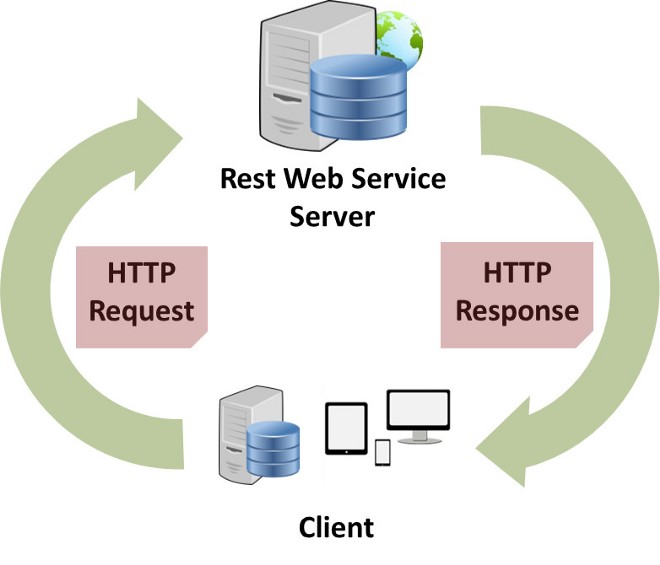
\includegraphics[width=0.5\linewidth]{images/design/clientserver.jpeg}}}%
    {\scriptsize%
     Source: \url{https://cdn-images-1.medium.com/max/660/1*EbBD6IXvf3o-YegUvRB_IA.jpeg}}
    \caption {A look at the server-client architecture with a RESTful interface.}
    \label{fig:design1}
\end{center}
\end{figure}


		\cleardoubleoddplainpage
		\label{part:Evaluation}
		\chapter{Evaluation}
\label{Evaluation}

Evaluation

This chapter is needed, when results from the previous chapters need to be systematically discussed. This is the case, when an implementation needs to be assessed, or the results of a case study or an experiment need to be interpreted.


- add the comparison between your approach and the other, in related work.

- add the test coverage statistics



		
		\cleardoubleoddplainpage
		\label{part:RelatedWork}
		\chapter{Related Work}
\label{RelatedWork}

In this chapter, we present some other approaches, which influenced our work. 

\section{SwiftCloud: a transactional system that brings geo-replication to the client}

Geo-replication of data into several data centres (DC) across the world is used in cloud platforms in order to improve availability and latency\cite{6}. This goal could be achieved even to a greater extent by storing some part of the data or even by replicating all of it at client machines. Thus, caching could be useful concerning the increasing availability of systems.

A system that integrates client- and server-side storage is called SwiftCloud, where the idea is to cache a subset of the objects from the DCs, and if the appropriate objects are in cache, then responsiveness is improved, and the operation without an internet connection is possible\cite{5}. The authors of the SwiftCloud state that it improves latency and throughput if it is compared to general geo-replication techniques. That is possible due to availability during faults thanks to automatic switch of DCs when the current one does not respond. Apart from that, SwiftCloud distributed object database is the first to provide fast reads and writes via a causally-consistent client-side local cache backed by the cloud. To provide the convergence of the data, SwiftCloud relies on CRDTs, which have rich confluent semantics\cite{7}.

\section{Legion: a framework, which enriches web applications}

A framework named Legion shows another exciting approach on how to address availability and scalability issues by using the cache at the client-side. The idea is to avoid a concept of a centralised infrastructure for mediating user interactions, as it causes unnecessarily high latency and hinders fault-tolerance and scalability\cite{8}. As an alternative, authors of Legion suggest client web applications to securely replicate data from servers and afterwards synchronise the data among the clients. This change makes the system less dependent on the server and, moreover, it reduces the latency of interactions among the clients. The guarantee of convergence between all of the replicas is possible due to CRDTs, introduced in \chapref*{Background}. 

\section{Developing web and mobile applications with offline usage experience}

Nowadays, applications with offline experience are becoming extremely popular. In this thesis, in \chapref*{Technologies} we presented an approach of developing web applications with the help of service workers and background synchronisation (they also go by the name of Progressive Web Applications [PWA]). It is a universal approach to create a cross-platform application that would work in web and on mobile devices. However, there are also other ways how the offline experience could be achieved. Sometimes, the process could become easier if specific frameworks are used. In the following subsections, we are going to describe the tools and techniques that are useful in this context. 


\subsection*{Polymer App Toolbox}

Polymer is a JavaScript library from Google, which helps to build web applications with the use of Web Components. The former concept represents a set of web platform APIs, which allow creating custom HTML tags to use in web pages\cite{16}. As web components are based on the latest web standards, and it eases the process of development. Polymer App Toolbox, in its turn, provides a collection of components to build PWAs with Polymer. However, the support of offline-experience is possible yet again due to Service Workers\cite{18}, which repeats the solution used in this thesis. Nevertheless, in contrast to the implementation offered in this thesis, working with Polymer App Toolbox requires additional knowledge of the Polymer framework. Currently, among the users of Polymer, apart from Google, there are such giants as Electronic Arts, IBM and Coca-Cola\cite{17}.

\subsection*{HTML5 Specification}

The specification of HTML5 contains some features that offer a possibility to build web applications that work offline. The solution to address this problem is to use SQL-based database API in order to be able to store data locally and to use an offline application HTTP cache to make sure about the availability of the application when there is no internet connection. The latter makes possible the following advantages: offline browsing, flexibility and a fast load of resources from the hard drive\cite{20}. However, from 2015 the application cache is considered to be deprecated and is recommended to be avoided\cite{21} in favour of Service Workers. Thus, for the implementation of WebCure, we favoured the approach of using a combination of a service worker and a Cache API.
 
\subsection*{Hoodie}

Hoodie is a framework, which eases the process of developing web and iOS applications. We will not cover all the features it offers and will only stop on it providing offline experience for applications that are developed using Hoodie. The documentation states that the framework is offline-first\cite{23}, which means that all the data is firstly stored locally and could be accessed without the internet connection. It is possible due to PouchDB database, which performs this work in the background\cite{24}. We will explore the process of how PouchDB works below.

\subsection*{localForage}

localForage is a JavaScript library, which provides the possibility to improve the offline-experience of web applications regarding storing data on the client-side. It uses IndexedDB, localStorage or WebSQL with a simple API. localForage sits on top of the data store layer and provides a range of methods to control the data. One of the useful benefits of it is that the data is not required to be explicitly converted into JSON format, as localForage does that automatically\cite{25}. localForage might be a useful library; however, as we already used IndexedDB Promised to work with IndexedDB database, we did not need to use anything heavier, such as localForage, primarily as it does not provide any fundamental differences in the approach.

\subsection*{PouchDB and CouchDB}

PouchDB represents an open-source JavaScript database, which is designed to build applications, which work well online and offline. To put it in a nutshell, PouchDB enables web applications to store the data locally, and, apart from that, eases the process of synchronisation with CouchDB-compatible servers. CouchDB, in its turn, is a database that is supported by a replication approach, which allows synchronising two or more servers, based on CouchDB. As there is a replication approach, it has its way of dealing with conflicts, which we explain next by following the description of the protocol offered by \citet{26}. 

\begin{lstlisting}[caption={A typical result of retrieving the item \textit{document} stored in CouchDB.}, label={lst:rwork1}]
{"_id":"document","_rev":"1-23202479633c2b380f79507a776743d5","a":1}
\end{lstlisting}

For every item stored in CouchDB, the database will add two extra properties: \textit{\_id} and \textit{\_rev}, which can be seen at \lstref*{lst:rwork1} that shows the result of getting an element named \textit{document} previously stored in the database. As we can see, the \textit{\_id} represents the name of the item, which is a custom name set by the user, while \textit{\_rev} represents the hash value, associated with the content. Afterwards, whenever we want to change the item \textit{document}, the same \textit{\_id} and \textit{\_rev} should be used.

\begin{lstlisting}[caption={Updating the value of item \textit{document} by adding \textit{b} into it.}, label={lst:rwork2}]
PUT /database/document
{"_id":"document","_rev":"1-23202479633c2b380f79507a776743d5","a":1, "b":2}
\end{lstlisting}

For example, to change the value of \textit{document} by adding \textit{b} into it, a simple PUT HTTP-request should be sent, as \lstref*{lst:rwork2} shows.

\begin{lstlisting}[caption={The result of requesting the updated version of \textit{document}}, label={lst:rwork3}]
GET /database/document
{"_id":"document","_rev":"2-c5242a69558bf0c24dda59b585d1a52b","a":1, "b":2}
\end{lstlisting}

The next retrieval of the \textit{document} will get us the result shown at \lstref*{lst:rwork3}.

As we can see, the \textit{\_rev} property got updated. In case the wrong revision is sent to update the document, the database will respond with an error.

\begin{lstlisting}[caption={Updating the value of item \textit{document} by adding \textit{d} into it.}, label={lst:rwork4}]
PUT /database/document
{"_id":"document","_rev":"2-c5242a69558bf0c24dda59b585d1a52b","a":1, "b":2, "d":4}
\end{lstlisting}

However, as our reader might have guessed, it is much more interesting, when we have more than one server. Let us assume that now we have two CouchDB servers. Imagine we try to update the \textit{document} once again with the values shown at \lstref*{lst:rwork4}.

\begin{lstlisting}[caption={The result of requesting the \textit{document} from CouchDB-1.}, label={lst:rwork5}]
GET /database/document
{"_id":"document","_rev":"3-2235fd4815b81b2da1b84159aba4006e", "a":1, "b":2, "d":4}
\end{lstlisting}

For example, let us say that it gets written to the first CouchDB server, which gives the response shown at \lstref*{lst:rwork5}.

\begin{lstlisting}[caption={The result of requesting the \textit{document} from CouchDB-2.}, label={lst:rwork6}]
GET /database/document
{"_id":"document","_rev":"2-c5242a69558bf0c24dda59b585d1a52b","a":1, "b":2}
\end{lstlisting}

However, the second CouchDB server still has the old data, as we can see at \lstref*{lst:rwork6}.

Ideally, the replication happens fastly, and both databases will synchronise and reach the same state. However, sometimes it might take a while. Moreover, if a client tries to update the document yet another time, there is a possibility that the update will go to the second server, which will reject the update, as \textit{\_rev} does not match any more. 

\begin{lstlisting}[caption={Updating the value of item \textit{document} by adding element \textit{e} and removing previously added element \textit{d}}, label={lst:rwork7}]
PUT /database/document
{"_id":"document","_rev":"3-2235fd4815b81b2da1b84159aba4006e", "a":1, "b":2, "e":5}
\end{lstlisting}

\begin{lstlisting}[caption={The demonstration of a conflict situation happening, when the \textit{\_rev} of sent operation and the one at the server do not match.}, label={lst:rwork8}]
{"error":"conflict","reason":"Document update conflict."}
\end{lstlisting}

As we mentioned earlier, the response of the second CouchDB server for the operation shown at \lstref*{lst:rwork7} will look like the one at \lstref*{lst:rwork8}.

\begin{lstlisting}[caption={Updating the value of item \textit{document} by adding element \textit{e} and removing previously added element \textit{d} after receiving the new \textit{\_rev} from the second CouchDB server.}, label={lst:rwork9}]
PUT /database/document
{"_id":"document","_rev":"2-c5242a69558bf0c24dda59b585d1a52b", "a":1, "b":2, "e":5}
\end{lstlisting}

However, there is another option to perform this update. We might have a strategy of getting the latest \textit{\_rev} first, which was \textit{"2-c5242a69558bf0c24dda59b585d1a52b"} at the second CouchDB server, and only then applying the update. So, the operation will look as at \lstref*{lst:rwork9}.

In case this PUT request goes to the second CouchDB server, then this operation will be successful, and now both servers will have different states, which creates a conflict situation. 
However, it is still an undesirable situation. Thus, there are the limitations that should be given a thought in the development process, which indeed make the process of creating the product based on CouchDB more complicated:
    \begin{itemize}
        \item {Making a change, do not request multiple GETs and POSTs;}
        \item {Do not update the \textit{\_rev} locally in the client without getting new data from the server before that;}
      \end{itemize}
      
Let us now summarize the advantages WebCure has due to using AntidoteDB and not CouchDB. 

First of all, since CouchDB ``blocks'' the possibility of updating the server's database without knowing the latest revision \textit{\_rev}, it already adds extra-work in the design and implementation of the protocol. Moreover, as we believe, it does not allow to perform concurrent updates. AntidoteDB, on the other hand, uses the concept of timestamps, which allows supporting causal consistency guarantees and, as it is not creating such restrictions on making updates, it has a massive advantage with the support of concurrent updates. 

\subsection*{Realm Mobile}

Realm Mobile is a framework, which makes integration of a client-side database for iOS and Android with a server-side, which offers the following features: real-time synchronisation, conflict resolution and event handling. This framework eases the process of developing applications with offline experience. The concept we are interested here is conflict-handling. In AntidoteDB, for this purpose, CRDTs are used. Realm Mobile maintains a good user experience in offline mode due to the rules they described for conflict resolution.
As they state, ``at a very high level the rules are as follows:

    \begin{itemize}
        \item {\textbf{Deletes always win.} If one side deletes an object, it will always stay deleted, even if the other side has made changes to it later on;}
        \item {\textbf{The last update wins.} If two sides update the same property, the value will end up as the last updated;}
        \item {\textbf{Inserts in lists are ordered by time.} If two items are inserted at the same position, the item that was inserted first will end up before the other item. It means that if both sides append items to the end of a list, they will end up in order of insertion time;}''\cite{22}
    \end{itemize}

The authors of the framework state that ``strong eventual consistency'' guarantees are reached\cite{22} with the approach mentioned above. Though, such way of conflict handling is not as flexible as CRDTs and has to be taken into account by the programmer at the stage of the development.

		\cleardoubleoddplainpage 
		\label{part:Conclusion}
		\chapter{Conclusion}
\label{Conclusion}

In this chapter, we will make a summary of our work and suggest some possibilities for future work.

\section{Summary}
\label{summary}

The work of this thesis mostly concentrated on designing such a client-server system, which would let replicating the data on a client machine. That would allow the user for offline operation at times, when there is no internet connection available, or when it is poor. Moreover, there are requirements for the system such as the possibility to maintain the data at client side as well, and synchronise it with a cloud storage server, when the mode of the client switches from offline to online. Additionally, after the system was designed, it was needed to be implemented, and its feasibility and performance should have been evaluated.

This task was achieved in a framework, which we named WebCure. Firstly, we designed a stable protocol for the communication between a client and a server. Then, we made a research on available technologies, which would allow us to implement the system in a way it is intended to work. Next, we developed a presentation application, which demonstrates the work of WebCure on an example of a set CRDT. After this step, we took a calendar application, which was already built based on AntidoteDB, and extended it to work with WebCure in order to evaluate the outcome. It turned out that, as expected, that the extended version of the calendar has a much shorter response time, better availability, while still keeping its original functionality and letting its users work both offline and online. 

\section{Future Work}
\label{futurework}

Different circumstances create uncertainty with the current design of the application. In this section, we would like to discuss these situations, while keeping the answers to them open for future improvements.

\section*{Missing acknowledgement}

In the current design of the WebCure, when a client is online and makes a request to the server with an update, the server sends back the acknowledgement, so the client knows that the requested operation was applied on the server side. However, there is a topic for discussion in this use case. Imagine that the server does not send back the acknowledgement. There are two possibilities:

\begin{itemize}
    \item {The update was applied on the server, but the connection failed when the acknowledgement was about to be sent back to the client;}
    \item {The update was not applied on the server, and the client did not receive the acknowledgement because of that.}
\end{itemize}

However, the problem is that a client does not know, which of the above situations happened. 

One of the solutions could be the following: it does not matter, whether the update was applied on the server or not. A client will send the update again, while it has not received an acknowledgement, regardless of what happens on the server's side. Nevertheless, in this case, updates must be uniquely identifiable, in order not to apply on the server the same update twice.

The other possibility is to have a double verification on the server side. For example, a client sends an update to the server. After that, the server should send a message back that it received an update. Next, if a client received that message with acknowledgement, it sends another message to the server that it is possible to apply the update. 

Though, the above information represents our thoughts on the problem, which is not necessarily a solution to it.  

\section*{Automatic updates of data at a client}

The current design of WebCure requires that after a client sends a request with an update to the server and receives an acknowledgement, it should then still send another read request in order to update the data on its side. However, this behaviour can be improved. For example, in some cases, it might be needed that a client acquires updates from the server automatically. To extend WebCure with such functionality, our suggestion would be to use Push Notifications feature\cite{32} of a service worker. The service worker can receive push messages from a server, even when the application is not active. It shows notifications to the user on their device even when the application is closed and still notify about the updates of the data on the server side.

\subsection*{Consistency guarantees}

\begin{figure}[!htb]
    \begin{center}
    \def\svgwidth{\linewidth}
    \input{images/architecture/future.pdf_tex}
    \caption {The case of breaking causal consistency guarantees in the current protocol.}
    \label{fig:final}
\end{center}
\end{figure}

In the current protocol design, there is a possibility to break the causality of applied operations, and that is what we would like to consider. There is a case with potential problems, which is illustrated in \figref*{fig:final}. There, a client reads the data by \textit{id} from the server, which has a \textit{value} associated with that \textit{id}, at the timestamp \textit{t\textsubscript{1}}. Once the client gets this data, it goes offline, performs some changes locally, and now it has the \textit{value'} associated with \textit{id}. Then, the connection gets back, and this update is sent to the server and applied. However, at this point, the connection breaks again, so the acknowledgement response from the server did not reach the client. That means, that at server side the update was applied and the element \textit{id} got its value changed to \textit{value'} at the timestamp \textit{t\textsubscript{2}}. Nevertheless, the client did not receive that information, the element \textit{id} at the client side still has local changes applied to it, which change its value to \textit{value'}. However, the interesting point here is that a client still has the timestamp \textit{t\textsubscript{1}}, stored on its side. Therefore, any further local updates performed at the client, once the internet connection is back again, will be sent to the server with information to apply them at the timestamp \textit{t\textsubscript{1}} and not \textit{t\textsubscript{2}}, how ideally it should be. The bad part here is that while our specific client is offline, some other clients could be communicating with the server at this time which means that the server could have received some updates from them as well. The current design of the protocol does not guarantee causal consistency in such situations. 

Discussing possible solutions, it all depends on the use case. Sometimes, freezing the client side functionality until it receives the acknowledgement from the server, might be acceptable. However, as it might take a long time, this is not a desirable solution. The other option is to check the states that are received after the server eventually responds (consisting of possible changes of the other clients) and find a solution by looking at the difference with the previous state, which is stored at the client side. However, this is a question, which is open for further investigation.

		{\hypersetup{linkcolor=black}
		\listoffigures
		\listoftables
		\listoftoc{loc}
		}
		\cleardoubleoddplainpage
		\bibliography{bibliography/references}
		

\end{document}